\documentclass [10pt] {beamer}
\usetheme      {Madrid}
\usecolortheme {rose}
\usefonttheme  {serif}

\setbeamertemplate {navigation symbols} {}
\setbeamertemplate {footline} [page number]
\setbeamertemplate {caption} [numbered]
\setbeamertemplate {itemize items} [circle]
\setbeamertemplate {enumerate items} [square]
\setbeamertemplate {theorems} [numbered]

\setbeamercolor {footnote mark} {fg = red}
\setbeamercolor {block title} {fg=black}

\setbeamersize {text margin left=10pt, text margin right=10pt}

\usepackage [T2A] {fontenc}
\usepackage [utf8] {inputenc}
\usepackage [english, main=russian] {babel}
\usepackage {mathrsfs}
\usepackage {graphicx}
\usepackage {ulem}
\usepackage {amsmath}
\usepackage {amssymb}
\usepackage {amsfonts}
\usepackage {amsthm}
\usepackage {indentfirst}
\usepackage {array}
\usepackage {multicol}
\usepackage {physics}
\usepackage {units}

\definecolor {forestgreen}   {rgb} {0.13, 0.55, 0.13}
\definecolor {fireenginered} {rgb} {0.81, 0.09, 0.13}
\definecolor {ceruleanblue}  {rgb} {0.16, 0.32, 0.75}

\newtheorem{proposition}{Утверждение}
\newtheorem{hypothesis}{Предположение}
\newtheorem{thm}{Теорема}

\title{Конденсат Бозе--Эйнштейна в нелинейных решётках: математическое и численное исследование}

\author{Лебедев Михаил Евгеньевич \\ \underline{Научный руководитель}: Алфимов Г. Л.}
\institute{
	Институт математики с вычислительным центром \\ УФИЦ РАН \\
	\medskip
	\textit{gloriouslair@gmail.com}
}
\date{Уфа -- 2021}

\begin{document}

% ************
% * SLIDE 01 *
% ************
\begin{frame}
	\titlepage
\end{frame}

% ************
% * SLIDE 02 *
% ************
\begin{frame}
	\frametitle{Актуальность работы}

	\begin{multicols}{2}
	[
	Одномерное уравнение Гросса--Питаевского (УГП):
	\begin{equation}
		i \Psi_t + \Psi_{xx} - U(x) \Psi + P(x) |\Psi|^2 \Psi = 0, \quad U(x), P(x) \in \mathbb{R}.
		\label{eq:gpe}
	\end{equation}
	В контексте теории конденсата Бозе--Эйнштейна (БЭК) описывает поведение <<сигарообразного>> конденсата; $\Psi(t, x)$ --- {\it \color{ceruleanblue} волновая функция}.
	]
	
	\begin{small}	
	\begin{itemize}
		\setlength\itemsep{5pt}
		\item БЭК --- это состояние вещества, возникающее при сверхнизких температурах.
		\item Предсказан в 1924 году в работах А. Эйнштейна и С. Бозе.
		\item Обнаружен в 1995 году в экспериментах Э. Корнелла, К. Вимана.
		\item 1995--2000-е: эксперименты с различными {\it \color{ceruleanblue} потенциалами удержания} $U(x)$, при этом $P(x) \equiv \pm 1$ (притяжение / отталкивание частиц).
		\item 2000--2010-е: появляются экспериментальные возможности генерации {\it \color{ceruleanblue} периодического псевдопотенциала} $P(x)$.
	\end{itemize}
	\end{small}
	\begin{figure}
		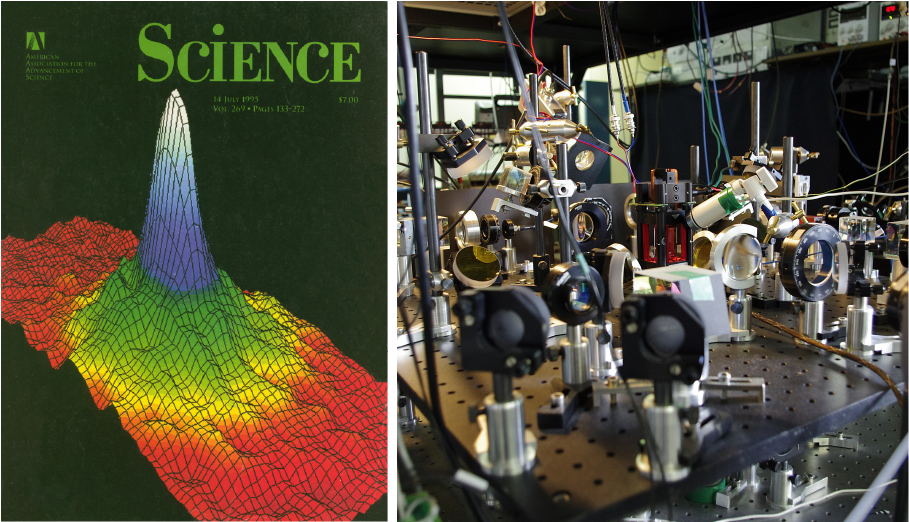
\includegraphics[scale=0.35]{pic/condensate.png}
	\end{figure}
	\end{multicols}
\end{frame}

% ************
% * SLIDE 03 *
% ************
\begin{frame}
	\frametitle{Актуальность работы}
	\framesubtitle{Резонанс Фешбаха, нелинейная решётка}
	
	\begin{columns}[T]
		\begin{column}{.5\textwidth}
			\begin{figure}
				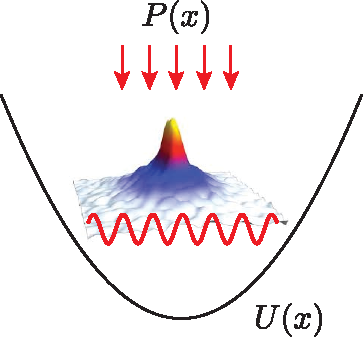
\includegraphics[width=1\textwidth]{pic/nonlinear lattice}
			\end{figure}
		\end{column}
		\begin{column}{.5\textwidth}
			$a_s = a_s(x)$ --- длина рассеяния частиц конденсата есть периодическая функция, $P(x) \sim a_s(x)$.
	
			\vspace{10pt}
	
			Механизмы создания нелинейной решётки:
			\begin{itemize}
				\item Магнитный резонанс Фешбаха. 
				\item Оптический резонанс Фешбаха.
			\end{itemize}
		\end{column}
	\end{columns}
\end{frame}

% ************
% * SLIDE 04 *
% ************
\begin{frame}
	\frametitle{Объект исследования}

	\begin{block}{Стационарные локализованные решения\footnotemark}
	 	Решение уравнения \eqref{eq:gpe} называется {\it \color{ceruleanblue} стационарным}, если оно представимо в виде
	 	\begin{equation}
			\Psi(t, x) = u(x) e^{-i \omega t}.	 		
	 	\end{equation}
		Стационарное УГП имеет вид неавтономного уравнения Дюффинга:
		\begin{equation}
			u_{xx} + Q(x) u + P(x) u^3 = 0, \quad Q(x) = \omega - U(x).
			\label{eq:stationary}
		\end{equation}
		Стационарное решение называется {\it \color{ceruleanblue} локализованным}, если $\lim \limits_{x \to \pm \infty} u(x) = 0$.
	\end{block}

	\begin{block}{Регулярные и сингулярные решения}
		Решение уравнения \eqref{eq:stationary} называется {\it \color{ceruleanblue} сингулярным}, если $\exists x_0, \lim \limits_{x \to x_0} u(x) = \infty$.
		Решение, не являющееся сингулярным, называется {\it \color{ceruleanblue} регулярным}.
	\end{block}
	
	\footnotetext{Также называемые {\it стационарными локализованными модами, СЛМ}}
\end{frame}

% ************
% * SLIDE 05 *
% ************
\begin{frame}
	\frametitle{Объект исследования}
	\framesubtitle{Устойчивые стационарные решения}
	
	\begin{block}{Устойчивые стационарные решения}
		Если решение неустойчиво, малые возмущения приводят к его разрушению при эволюции.
		\begin{equation}
			\Psi(t, x) = \left( u(x) + \widetilde{U}(t, x) \right) e^{i \omega t}; \quad |\widetilde{U}(t, x)| \ll 1.
		\end{equation}
		Именно устойчивые решения важны с точки зрения различных физических приложений.
	\end{block}
\end{frame}

% ************
% * SLIDE 06 *
% ************
\begin{frame}
	\frametitle{Известные результаты}
	\framesubtitle{Исследование специальных классов}
	
	\begin{small}
	\begin{enumerate}
		\setlength\itemsep{5pt}
		\item[1.] Y. V. Kartashov, B. A. Malomed, L. Torner, ``Solitons in nonlinear lattices'' // Rev. Mod. Phys., Vol. {\bf 83}, P. 247 (2011).
			\begin{itemize}
				\item Исчерпывающий обзор физических моделей, в которых возникает переменный псевдопотенциал $P(x)$.
			\end{itemize}
		\item[2.] H. Sakaguchi, B. A. Malomed // Phys. Rev. E, Vol.{\bf 72}, P. 046610 (2005).
			\begin{itemize}
				\item Рассмотрена модель $U(x) \equiv 0$, $P(x) = A - \cos 2x$.
				\item Исследована устойчивость фундаментального решения методом \underline{вариационной аппроксимации}.
			\end{itemize}
		\item[3.] Bludov, Y. V., and V. V. Konotop // Phys. Rev. A, Vol. {\bf 74}, P. 043616 (2006).
			\begin{itemize}
				\item Рассмотрен БЭК смеси бозонов и фермионов; $U(x)$, $P(x)$ --- периодические функции.
				\item Произведен численный анализ \underline{простейших решений} задачи.
			\end{itemize}
	\end{enumerate}
	\end{small}
\end{frame}

% ************
% * SLIDE 07 *
% ************
\begin{frame}
	\frametitle{Известные результаты}
	\framesubtitle{Полное описание всех имеющихся СЛМ}
	
	\begin{small}
	\begin{enumerate}
		\setlength\itemsep{5pt}
		\item[1.] G. L. Alfimov, D. A. Zezyulin // Nonlinearity, Vol. {\bf 20}, P. 2075--2092 (2007).
			\begin{itemize}
				\item Рассмотрен случай $U(x) = Ax^2$, $P(x) \equiv \pm 1$.
				\item Предложен метод <<доказательных вычислений>>, позволяющий гарантировать нахождение \underline{всех} регулярных решений.
			\end{itemize}
		\item[2.] G. L. Alfimov, I. V. Barashenkov, A. P. Fedotov, V. V. Smirnov, D. A. Zezyulin // Physica D, Vol. {\bf 397}, P. 39--53 (2019).
			\begin{itemize}
				\item Обобщение задача на случай системы из нескольких связанных уравнений Гросса--Питаевского.
			\end{itemize}
		\item[3.] G. L. Alfimov, A. I. Avramenko // Physica D, Vol. {\bf 254}, P. 29--45, (2013).
			\begin{itemize}
				\item Рассмотрен случай $U(x)$ -- периодическая функция, $P(x) \equiv -1$.
				\item Предложены достаточные условия, допускающие исчерпывающее описание \underline{всех} ограниченных решений.
				\item Показана возможность \underline{кодирования} решений.
			\end{itemize}
		\item[4.] G. L. Alfimov, P. P. Kizin, D. A. Zezyulin // Discrete and Continuous Dynamical Systems --- Series B, Vol. {\bf 22}, P. 1207--1229 (2017).
			\begin{itemize}
				\item Разработан алгоритм, позволяющий по коду решения численно построить его профиль.
			\end{itemize}
	\end{enumerate}
	\end{small}
\end{frame}

% *************
% * SLIDE 07b *
% *************
\begin{frame}
	\frametitle{Известные результаты}
	\framesubtitle{Полное описание всех имеющихся СЛМ}
	
	\begin{small}
	\begin{enumerate}
		\setlength\itemsep{5pt}
		\item[1.] Ch. Zanini, F. Zanolin // Complexity, Vol. {\bf 2018}, Article ID 2101482 (2018).
		\item[2.] Ch. Zanini, F. Zanolin // Advanced Nonlinear Studies, Vol. {\bf 12}, No. 3, P. 481--499 (2012).
			\begin{itemize}
				\item Доказывается существование некоторых типов решений в близких задачах.
				\item Решения могут быть полностью описаны в терминах нелинейной динамики.
				\item Подход основан на топологических аргументах.
			\end{itemize}
	\end{enumerate}
	\end{small}
\end{frame}

% ************
% * SLIDE 08 *
% ************
\begin{frame}
	\frametitle{Цели и задачи}
	
	\begin{equation*}
		i \Psi_t + \Psi_{xx} - U(x) \Psi + P(x) |\Psi|^2 \Psi = 0.
	\end{equation*}
	
	\begin{enumerate}
		\item[1.] Обобщение метода кодировки СЛМ на случай периодических $U(x)$, $P(x)$.
			\begin{itemize}
				\item Сформулировать достаточные условия возможности кодирования.
				\item Предложить способ проверки достаточных условий.
			\end{itemize}
		\item[2.] Исследовать множество СЛМ с периодическим $P(x)$, и $Q(x) \equiv 0$ (принципиально нелинейное взаимодействие).
			\begin{itemize}
				\item Описание решений.
				\item Исследование устойчивости.
			\end{itemize}
		\item[3.] Влияние периодического $P(x)$ на множество СЛМ в случае $U(x) = A x^2$ (бесконечная потенциальная яма).
			\begin{itemize}
				\item Связь со случаем $P(x) \equiv -1$.
				\item Исследование устойчивости.
			\end{itemize}
	\end{enumerate}
\end{frame}

% ************
% * SLIDE 09 *
% ************
\begin{frame}
	\begin{center}
		\LARGE Глава 1. Математические результаты \\ о регулярных и сингулярных решениях уравнения $u_{xx} + Q(x) u + P(x) u^3 = 0$
	\end{center}
\end{frame}

% ************
% * SLIDE 10 *
% ************
\begin{frame}
	\frametitle{Общие утверждения о регулярности решений}

	\begin{equation}
		u_{xx} + Q(x) u + P(x) u^3 = 0.
		\label{eq:proposition}
	\end{equation}

	\begin{proposition}
		Пусть $\forall x \in \mathbb{R}$, функции $Q(x)$, $P(x) \in C^1(\mathbb{R})$, причем
		\begin{enumerate}
			\item[(а)] $P(x) \ge P_0 > 0$, $|P'(x)| \le \widetilde{P}$;
			\item[(б)] $Q(x) \ge Q_0$, $|Q'(x)| \le \widetilde{Q}$;
		\end{enumerate}
		тогда решение задачи Коши для уравнения \eqref{eq:proposition} c произвольными начальными условиями $(u_0, u_0')$ {\bf регулярно} и может быть продолжено на всю действительную ось $\mathbb{R}$.
		\label{prop:regular}
	\end{proposition}

	\medskip
	
	\begin{proposition}
		Пусть $\forall x \in \mathbb{R}$ выполняются условия: $P(x) \le P_0 < 0$, $Q(x) \le Q_0 < 0$, тогда все решения уравнения \eqref{eq:proposition} {\bf сингулярны}, за исключением нулевого решения.
		\label{prop:singular}
	\end{proposition}
	
\end{frame}

% ************
% * SLIDE 11 *
% ************
\begin{frame}
	\frametitle{Семейства сингулярных решений}

	\begin{proposition}
		Пусть $\exists x_0$, $P(x_0) < 0$, $\Omega$ --- некоторая окрестность точки $x_0$, причём $Q(x) \in C^2(\Omega)$ и $P(x) \in C^4(\Omega)$, тогда существуют два $C^1$~--~гладких однопараметрических семейства решений уравнения \eqref{eq:proposition}, {\bf сингулярных} в точке $x_0$, связаных между собой симметрией $u \to -u$ и имеющих разложения:
		\begin{equation}
			\pm u(x) = \frac{\sqrt{2}} \eta + A_0 + A_1 \eta + A_2 \eta^2 + A_3 \eta^3 \ln|\eta| + C \eta^3 + A_4 	\eta^4 \ln|\eta| + \ldots,
			\label{eq:series}
		\end{equation}
 		где $\eta = x - x_0$.
		Каждое из этих семейств можно запараметризовать свободной переменной $C \in \mathbb{R}$.
	\end{proposition}

	\begin{small}
		\begin{eqnarray*}	
			&& A_0 = \frac{\sqrt{2}}3P_1, \quad A_1 = \frac{\sqrt{2}} 3P_2 + \frac{\sqrt{2}} 6Q_0 + \frac{2\sqrt{2}} 9P_1^2; \\[2mm]
			&& A_2 = \frac{2\sqrt{2}} 3P_2 P_1 + \frac{7\sqrt{2}}{27} P_1^3 + \frac{\sqrt{2}} 6Q_0 P_1 + \frac{\sqrt{2}} 4Q_1 + \frac{\sqrt{2}} 2P_3 \dots
		\end{eqnarray*}
	\end{small}	
\end{frame}

% ************
% * SLIDE 12 *
% ************
\begin{frame}
	\frametitle{Результаты 1-й главы}
	
	\begin{table}
		\begin{tabular}{ | m{70pt} | l || m{190pt} | }
			\hline
			$P(x)$ & $Q(x)$ & \\
			\hline
			$P(x) > 0$ & --- & Все решения продолжаются на действительную ось, сингулярные решения отсутствуют. \\
			\hline
			$P(x) < 0$ хотя бы в одной точке $x = x_0$ & --- & Имеется пара однопараметрических семейств решений, коллапсирующих в точке $x = x_0$ и связанных симметрией $u~\to~-u$. \\
			\hline
			$P(x) < 0$ & $Q(x) < 0$ & Все решения сингулярны за исключением нулевого решения. \\
			\hline
			$P(x)$ знакопеременна & --- & {\color{ceruleanblue} Сингулярность решений является типичным поведением}. Это позволяет при некоторых дополнительных ограничениях применить {\it метод исключения сингулярных решений} и {\color{ceruleanblue} классифицировать} оставшиеся {\it регулярные решения} в терминах символической динамики. \\
			\hline
		\end{tabular}
	\end{table}
\end{frame}

% ************
% * SLIDE 13 *
% ************
\begin{frame}
	\begin{center}
		{\LARGE Глава 2. Аппарат классификации стационарных решений, $$P(x) <> 0$$}
	\end{center}
\end{frame}

% ************
% * SLIDE 14 *
% ************
\begin{frame}
	\frametitle{Классификация}
	\framesubtitle{Основные определения}
	
	\begin{equation}
		u_{xx} + Q(x) u + P(x) u^3 = 0, \quad Q(x + L) = Q(x), \quad P(x + L) = P(x).
		\label{eq:classification}
	\end{equation}

	\begin{block}{Множества $\mathscr{U}_L^{\pm}$}
	$\mathscr{U}_L^{\pm} = \{ (u_0, u_0') \in \mathbb{R}^2$ | решение задачи Коши для уравнения \eqref{eq:classification} с НУ $(u_0, u_0')$ регулярно на $[0, {\pm} L] \}$, $\mathscr{U}_L = \mathscr{U}_L^+ \cap \mathscr{U}_L^-$.
	\end{block}

	\begin{block}{Отображение Пуанкаре $\mathcal{P}: \mathbb{R}^2 \to \mathbb{R}^2$}
		$\mathcal{P} (u_0,u_0') = (u(L), u'(L))$, где $u(x)$ --- решение с НУ $(u_0, u_0')$.
	\end{block}

	$$\vb{p} = (u_0, u_0') \in \mathscr{U}_L^+ = \mathrm{dom}(\mathcal{P}), \quad \mathcal{P}(\vb{p}) = \vb{q} \in \mathscr{U}_L^- = \mathrm{dom}(\mathcal{P}^{-1}).$$

	\begin{block}{Орбита}
		Последовательность точек $\{ p_n \}$ таких, что $\mathcal{P}(p_n) = p_{n+1}$.
	\end{block}
\end{frame}

% ************
% * SLIDE 15 *
% ************
\begin{frame}
	\frametitle{Классификация}
	\framesubtitle{Кусочно-постоянный псевдопотенциал}
	
	Проиллюстрируем на примере уравнения
	\begin{equation}
		u_{xx} - u + \eta(x) u^3 = 0,
		\label{eq:piecewise}
	\end{equation}
	
	$\eta(x)$ --- кусочно-постоянный псевдопотенциал с периодом $L = L_* + L_0$:
	\begin{equation*}
		\eta(x) = \left\{
			\begin{array}{rl}
				-1, &  x \in [0; L_*); \\[1.5mm]
				+1, & x \in [L_*; L_* + L_0).
			\end{array}
		\right.
	\end{equation*}
	
	\begin{figure}
		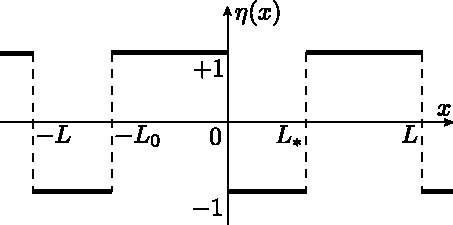
\includegraphics[width = 0.5\textwidth]{pic/piecewise constant.pdf}
	\end{figure}
\end{frame}

% ************
% * SLIDE 16 *
% ************
\begin{frame}
	\frametitle{Кусочно-постоянный псевдопотенциал}
	\framesubtitle{Переключение режимов: фазовые портреты}
	
	\begin{figure}
		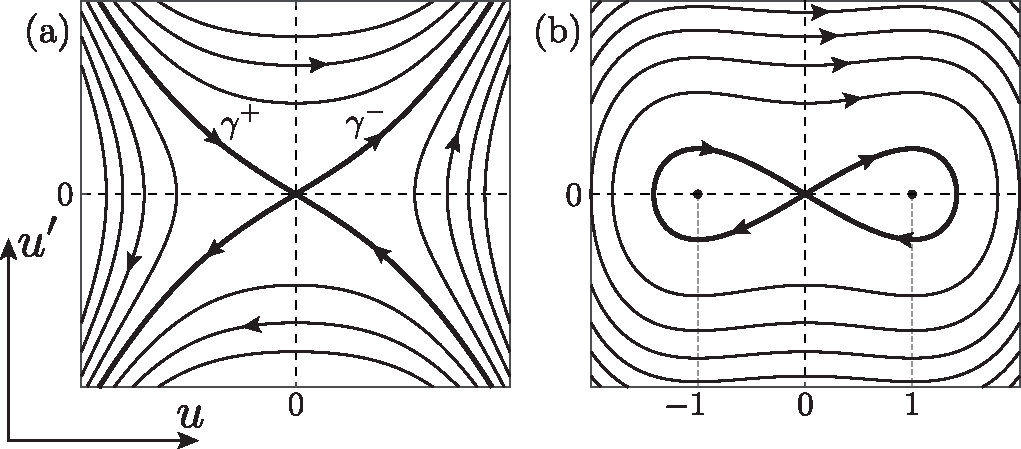
\includegraphics[width = \textwidth]{pic/phase portraits.pdf}
		\caption{Фазовые портреты: (a) $u - u - u^3 = 0$, (b) $u - u + u^3 = 0$. Уравнение (a) связано с отображением $\mathcal{P}_*$, уравнение (b) связано с отображением $\mathcal{P}_0$.}
	\end{figure}
	
	\begin{center}
		Отображение $\mathcal{P}$ можно представить в виде композиции $\mathcal{P} = \mathcal{P}_0 \mathcal{P}_*$.
	\end{center}
\end{frame}

% ************
% * SLIDE 17 *
% ************
\begin{frame}
	\frametitle{Классификация}
	\framesubtitle{Сканирование плоскости начальных данных}
	
	\begin{figure}
		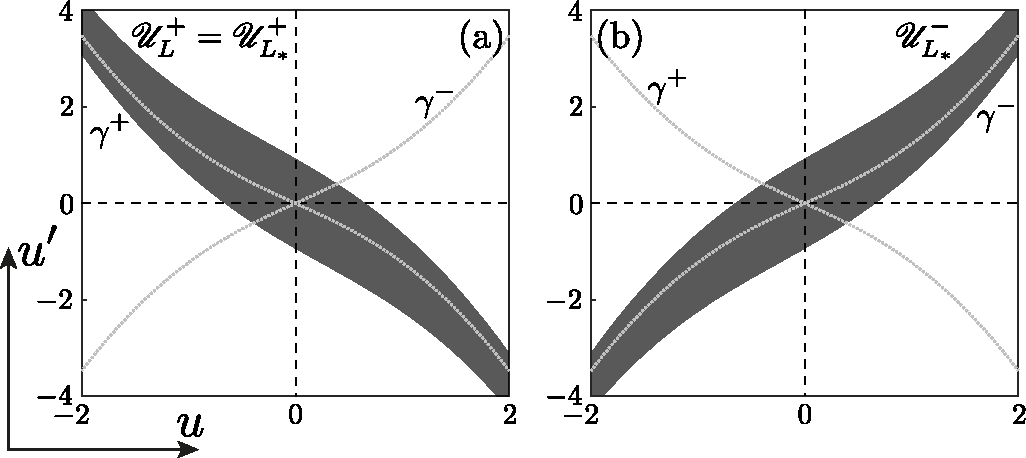
\includegraphics[width = \textwidth]{pic/Poincare map domain for piecewise singular equation.pdf}
		\caption{Области определения отображений, полученные численно путём сканированием плоскости начальных данных (a) $\mathscr{U}_L^+$, (b) $\mathcal{P}_*(\mathscr{U}_L^+) = I \mathscr{U}_L^+$, где $I$ --- отражение относительно оси $u'$.}
	\end{figure}
\end{frame}

% ************
% * SLIDE 18 *
% ************
\begin{frame}
	\frametitle{Кусочно-постоянный псевдопотенциал}
	\framesubtitle{Отображение сепаратрисы, $\mathcal{P}_0(\gamma_-)$}
	
	\begin{columns}[T]
		\begin{column}{.5\textwidth}
			\begin{figure}
			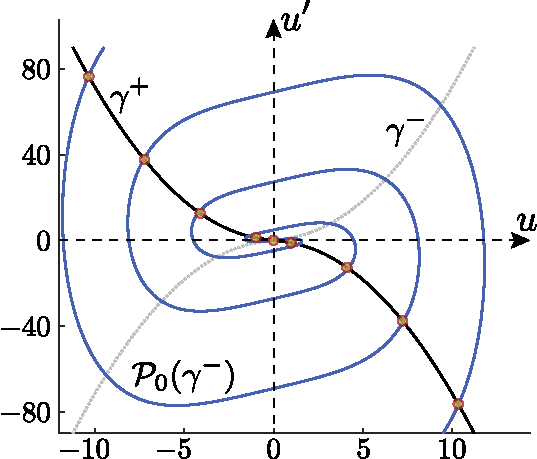
\includegraphics[width = 1\textwidth]{pic/separatrix map with numerical computations.pdf}
			\caption{$\mathcal{P}_0(\gamma^-)$ (синий) --- бесконечная спираль; точки пересечения $\mathcal{P}_0(\gamma^-) \cap \gamma^+$ согласно \eqref{eq:intersections} (жёлтый).}
			\end{figure}
		\end{column}
		\begin{column}{.5\textwidth}
			\begin{proposition}
				$\mathcal{P}_0 (\gamma^-)$ есть бесконечная спираль, она пересекает $\gamma^+$ в точках $\{0\} \cup \{u_{\pm n}\}$, $n \in \mathbb{N}$,
				\begin{equation}
					u_{\pm n} = \pm \dfrac{2 x_{n - 1}}{\sqrt[4]{2} L_0} + \mathcal{O}(H_0^{\nicefrac{-1}{4}});
					\label{eq:intersections}
				\end{equation}
				$H_0 \to \infty$, где значения $x_n$ определяются по формуле
				\begin{equation*}
					x_n = \mathrm{cn}^{-1} \left( 2^{\nicefrac{-1}{4}}, 2^{\nicefrac{-1}{2}} \right) + \mathrm{K}(2^{\nicefrac{-1}{2}}) n.
				\end{equation*}
			\end{proposition}
			
			$\textrm{K}$ --- полный эллиптический интеграл 1-го рода; \\
			$\textrm{cn}^{-1}$ --- обратный эллиптический косинус.
		\end{column}
	\end{columns}
\end{frame}

% ************
% * SLIDE 19 *
% ************
\begin{frame}
	\frametitle{Кусочно-постоянный псевдопотенциал}
	\framesubtitle{Множество $\mathscr{U}_L = \mathscr{U}_L^+ \cap \mathscr{U}_L^-$}
	
	\begin{figure}
	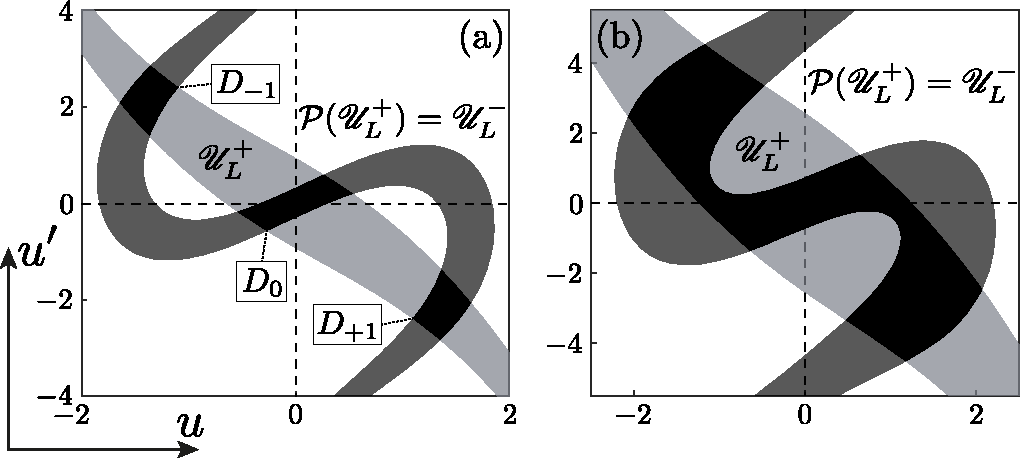
\includegraphics[width = \textwidth]{pic/island set for piecewise equation.pdf}
	\caption{
		Множества $\mathscr{U}_L^+$ (светло-серый), $\mathscr{U}_L^-$ (тёмно-серый), и их пересечение $\mathscr{U}_L$ (чёрный) для уравнения \eqref{eq:piecewise}; (a) $(L_*, L_0) = (2, 1)$; (b) $(L_*, L_0) = (1.3, 1)$.
	}
	\end{figure}
\end{frame}

% ************
% * SLIDE 20 *
% ************
\begin{frame}
	\frametitle{Классификация}
	\framesubtitle{Островное множество}
	
	\begin{columns}[T]
		\begin{column}{.47\textwidth}
			\begin{block}{Остров}
				Криволинейный четырёхугольник, ограниченный двумя парами монотонных кривых $\alpha^{\pm}$, $\beta^{\pm}$.
			\end{block}		
			\begin{figure}
			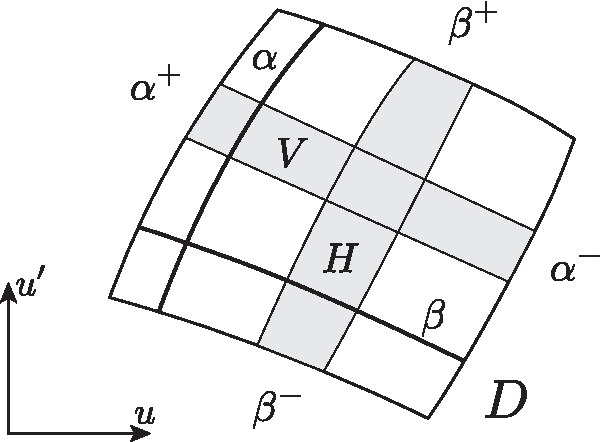
\includegraphics[height = 0.4\textheight]{pic/curves and strips.pdf}
			\caption{Остров $D$, h-кривая $\alpha$, v-кривая $\beta$, h-полоса $H$, v-полоса $V$.}
			\end{figure}
		\end{column}
		\begin{column}{.46\textwidth}
			\begin{block}{Островное множество}
				Набор островов на плоскости начальных условий $\bigcup_{k \in S} D_k$.
			\end{block}
			\vspace{10pt}
			\begin{figure}
			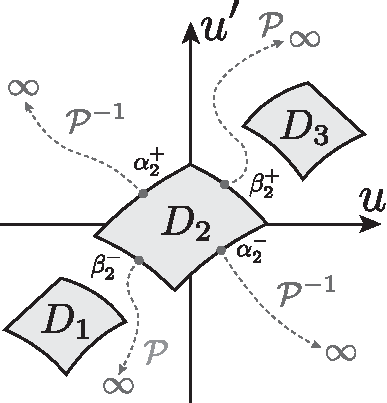
\includegraphics[height = 0.4\textheight]{pic/island set.pdf}
			\caption{Пример островного множества, $\mathscr{U}_L = \{ D_1, D_2, D_3 \}$.}
			\end{figure}
		\end{column}
	\end{columns}
\end{frame}

% ************
% * SLIDE 21 *
% ************
\begin{frame}
	\frametitle{Кодирование решений}
	
	Пусть множество $\mathscr{U}_L$ --- островное, $\mathscr{U}_L = \bigcup_{k \in S} D_k$.
	
	\vspace{5pt}
	
	\underline{Орбите} регулярного решения $\{ \vb{p}_k \}$ можно поставить в соответствие \underline{последовательность} символов $\{ \dots, i_{-1}, i_0, i_{+1}, \dots \}$, $\vb{p}_k \to i_k, \, \vb{p}_k \in D_{i_k}$.
	\begin{figure}
	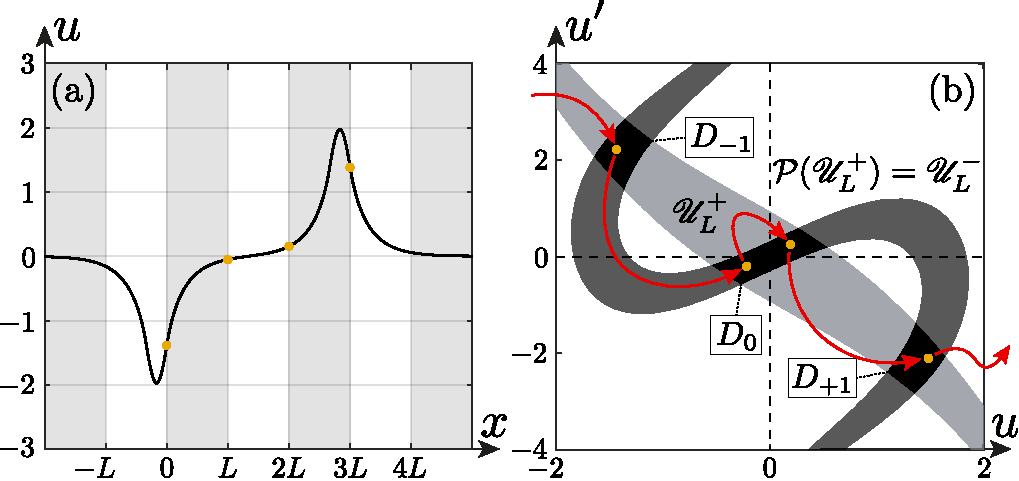
\includegraphics[width = 0.85\textwidth]{pic/solution and orbit on the phase plane.pdf}
	\caption{
		Локализованное решение (a) имеет код $\{ \dots, 0, -1, 0, 0, +1, 0, \dots \}$; (б) точки $\vb{p}_k$ на плоскости начальных данных; $(L_*, L_0) = (2, 1)$.
	}
	\end{figure}
\end{frame}

% ************
% * SLIDE 22 *
% ************
\begin{frame}
	\frametitle{Взаимно-однозначное кодирование: $\mathrm{dom}(\mathcal{P}^{-2})$}
	
	\begin{figure}
	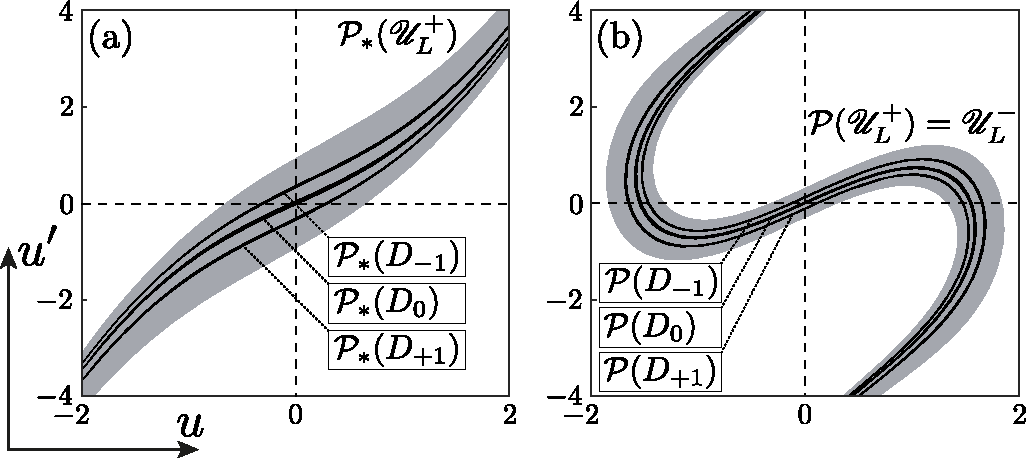
\includegraphics[width = 1\textwidth]{pic/Poincare map of islands for piecewise equation.pdf}
	\caption{
		(a) $\mathcal{P}_*$-образ островного множества (чёрный) внутри $\mathcal{P}_*(\mathscr{U}_L^+)$ (серый); (b) $\mathcal{P}$-образ островного множества (чёрный) внутри $\mathscr{U}_L^-$ (серый).
		Уравнение \eqref{eq:piecewise} с параметрами $(L_*, L_0) = (2, 1)$.
	}
	\end{figure}
\end{frame}

% ************
% * SLIDE 23 *
% ************
\begin{frame}
	\frametitle{Взаимно-однозначное кодирование: h-полосы}
	
	\begin{columns}
		\begin{column}{.5\textwidth}
			\begin{figure}
			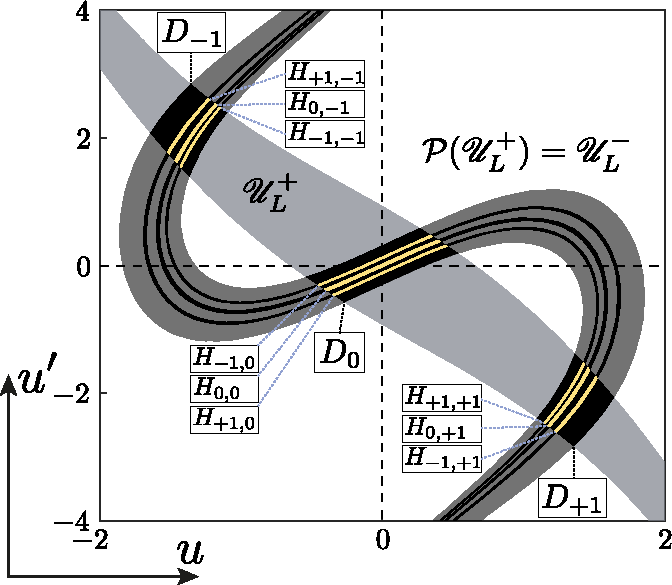
\includegraphics[width = 1\textwidth]{pic/h-strips for piecewise equation.pdf}
			\caption{Множества $H_{ij}$ (жёлтый) для уравнения \eqref{eq:piecewise} с параметрами $(L_*, L_0) = (2, 1)$.}
			\end{figure}
		\end{column}
		\begin{column}{.5\textwidth}
			Множество $\mathscr{U}_L = \bigcup_{k \in S} D_k$ --- островное.
		
			\vspace{5pt}
		
			\begin{equation*}
				\forall i, j, \, H_{ij} = \mathcal{P}(D_i) \cap D_j \neq \varnothing	
			\end{equation*}

			\vspace{5pt}
			
			В точках $\vb{p} \in H_{ij}$ определены отображения $\mathcal{P}$, $\mathcal{P}^{-1}$ и $\mathcal{P}^{-2}$.
			
			\vspace{10pt}
			
			Границы $H_{ij}$ монотонны, значит $H_{ij}$ представляют собой \underline{h-полосы}.
		\end{column}
	\end{columns}
\end{frame}

% ************
% * SLIDE 24 *
% ************
\begin{frame}
	\frametitle{Взаимно-однозначное кодирование: v-полосы}
	
	\begin{columns}
		\begin{column}{.5\textwidth}
			\begin{figure}
			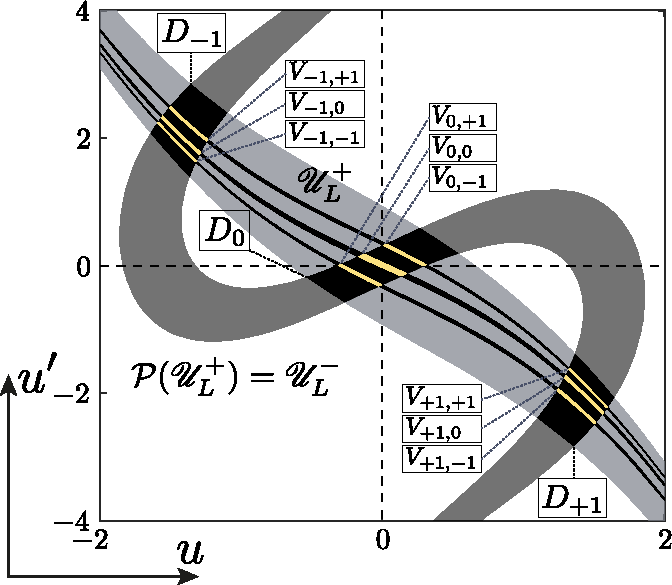
\includegraphics[width = 1\textwidth]{pic/v-strips for piecewise equation.pdf}
			\caption{Множества $V_{ij}$ (жёлтый) для уравнения \eqref{eq:piecewise} с параметрами $(L_*, L_0) = (2, 1)$.}
			\end{figure}
		\end{column}
		\begin{column}{.5\textwidth}
			Множество $\mathscr{U}_L = \bigcup_{k \in S} D_k$ --- островное.
		
			\vspace{5pt}
		
			\begin{equation*}
				\forall i, j, \, V_{ij} = \mathcal{P}^{-1}(D_j) \cap D_i \neq \varnothing	
			\end{equation*}

			\vspace{5pt}
			
			В точках $\vb{p} \in V_{ij}$ определены отображения $\mathcal{P}$, $\mathcal{P}^2$ и $\mathcal{P}^{-1}$.
			
			\vspace{10pt}
			
			Границы $V_{ij}$ монотонны, значит $V_{ij}$ представляют собой \underline{v-полосы}.
		\end{column}
	\end{columns}
\end{frame}

% ************
% * SLIDE 25 *
% ************
\begin{frame}
	\frametitle{Формирование точечного множества}
	
	\begin{columns}
		\begin{column}{.5\textwidth}
			\begin{figure}
			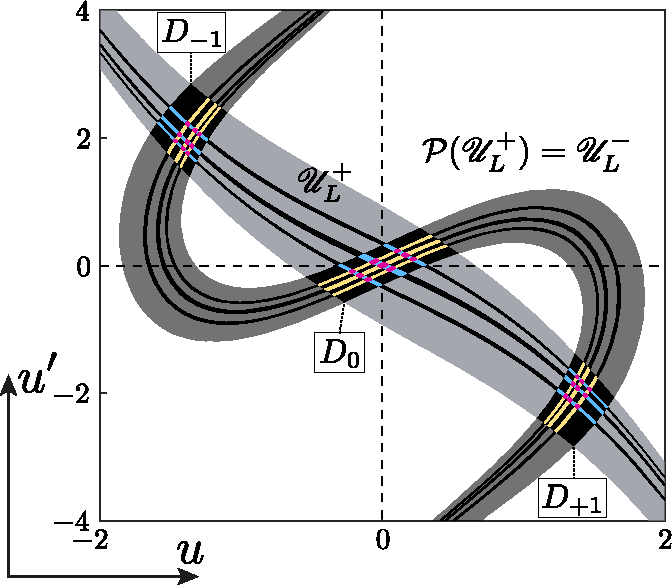
\includegraphics[width = 1\textwidth]{pic/h- and v-strips for piecewise equation.pdf}
			\caption{
				Множества $\mathscr{H}_1 = \bigcup_{i,j \in S} H_{ij}$ (жёлтый), $\mathscr{V}_1 = \bigcup_{i,j \in S} V_{ij}$ (синий) и их пересечение $\mathscr{H}_1 \cap \mathscr{V}_1$ (розовый).
			}
			\end{figure}
		\end{column}
		\begin{column}{.5\textwidth}
		\begin{center}
			Когда продолжение этого процесса приводит к формированию точечного множества?
			
			\vspace{15pt}
			
			Действие отображения $\mathcal{P}$ на множестве $\mathscr{U}_L$ происходит по схеме подковы Смейла?
			
			\vspace{15pt}
			
			Существует взаимно-однозначное отображение между кодами и орбитами решений?
		\end{center}
		\end{column}
	\end{columns}
\end{frame}

% ************
% * SLIDE 26 *
% ************
\begin{frame}
	\frametitle{Формализация, предположения}
	
	\begin{equation}
		u_{xx} + Q(x) u + P(x) u^3 = 0, \quad Q(x + L) = Q(x), \quad P(x + L) = P(x).
		\label{eq:formalization}
	\end{equation}
	
	\begin{hypothesis}[Островное множество]
		Для уравнения \eqref{eq:formalization} множество $\mathscr{U}_L$ представляет из себя набор островов, $\mathscr{U}_L = \bigcup_{i \in S} D_i$.
	\end{hypothesis}

	\begin{hypothesis}[Отображение полос]
		Для любых $i, j \in S$ и для любой h-полосы $H \in D_i$ её $\mathcal{P}$-образ $\widetilde{H}_j = \mathcal{P}(H) \cap D_j$ есть $\mathrm{h}$-полоса, и существует $\mu > 1$, что
		\begin{equation}
			d_{\mathrm{h}}(\widetilde{H}_j) \le (1/\mu) d_{\mathrm{h}}(H).
		\end{equation}
		Для любых $i, j \in S$ и для любой v-полосы $V \in D_j$ её $\mathcal{P}$-прообраз $\widetilde{V}_i = \mathcal{P}^{-1}(V) \cap D_i$ есть $\mathrm{v}$-полоса, и существует $\nu > 1$, что
		\begin{equation}
			d_{\mathrm{v}}(\widetilde{V}_i) \le (1/\nu) d_{\mathrm{v}}(V).
		\end{equation}
	\end{hypothesis}
\end{frame}

% ************
% * SLIDE 27 *
% ************
\begin{frame}
	\frametitle{Теорема о кодировании решений}
	
	$\mathcal{O}$ --- множество всех орбит регулярных решений уравнения \eqref{eq:formalization}.

	\vspace{10pt}

	$\mathcal{S}$ --- множество бесконечных последовательностей из символов, соответствующих компонентам связности множества $\mathscr{U}_L$.
	
	\vspace{10pt}
	
	Определим отображение $\mathcal{C}: \mathcal{O} \to \mathcal{S}$, $\vb{r} \in \mathcal{O}$, $\vb{r} = \{ \vb{p}_k \}$, $\mathcal{C}(\vb{r}) = \vb{s} \in \mathcal{S}$, $\vb{s} = \{ i_k \}$ такая, что $i_k$ есть номер компоненты $D_{i_k}$, содержащей $\vb{p}_k$. 

	\vspace{10pt}
	
	\begin{thm}[О кодировании решений]
		Пусть предположения I, II верны, тогда $\mathcal{C}$ есть гомеоморфизм топологических пространств $\mathcal{O}$ и $\mathcal{S}$.
	\end{thm}
	
	\vspace{10pt}
	
	\begin{center}
		Как проверить предположения?
	\end{center}
\end{frame}

% ************
% * SLIDE 28 *
% ************
\begin{frame}
	\frametitle{Проверка гипотез: численная процедура}
	
	\begin{equation*}
		\mathcal{P}(\vb{q}) = \mathcal{P}(\vb{p}) + D \mathcal{P}_{\vb{p}} (\vb{q} - \vb{p}) + o(||\vb{q} - \vb{p}||).
	\end{equation*}
	
	\begin{thm}[Об отображении h-полос]
		\begin{itemize}
			\item Если знаки $a_{mn}$ в матрице $D \mathcal{P}_{\vb{p}} = (a_{mn})$, $\vb{p} \in V_{ij}$, удовлетворяют \underline{некоторым условиям}, тогда $\mathcal{P}$ отображает h-полосы в h-полосы.
			\item Если для оператора $D \mathcal{P}_{\vb{p}} = (a_{mn})$ для всех $\vb{p} \in V_{ij}$ имеет место оценка $|a_{11}| \ge \mu > 1$ ($\exists \mu$), тогда $\mathcal{P}$ \underline{сжимает} h-полосы.
		\end{itemize}
	\end{thm}
	\begin{equation*}
		\mathcal{P}^{-1}(\vb{q}) = \mathcal{P}^{-1}(\vb{p}) + D \mathcal{P}^{-1}_{\vb{p}} (\vb{q} - \vb{p}) + o(||\vb{q} - \vb{p}||).
	\end{equation*}
	\begin{thm}[Об отображении v-полос]
		\begin{itemize}
			\item Если знаки $b_{mn}$ в матрице $D \mathcal{P}_{\vb{q}}^{-1} = (b_{mn})$, $\vb{q} \in H_{ij}$, удовлетворяют \underline{некоторым условиям}, тогда $\mathcal{P}^{-1}$ отображает v-полосы в v-полосы.
			\item Если для оператора $D \mathcal{P}_{\vb{q}}^{-1} = (b_{mn})$ для всех $\vb{q} \in H_{ij}$ имеет место оценка $|b_{22}| \ge \nu > 1$ ($\exists \nu$), тогда $\mathcal{P}^{-1}$ \underline{сжимает} v-полосы.
		\end{itemize}
	\end{thm}
\end{frame}

% ************
% * SLIDE 29 *
% ************
\begin{frame}
	\frametitle{Проверка гипотез: иллюстрация}
	
	\begin{figure}
	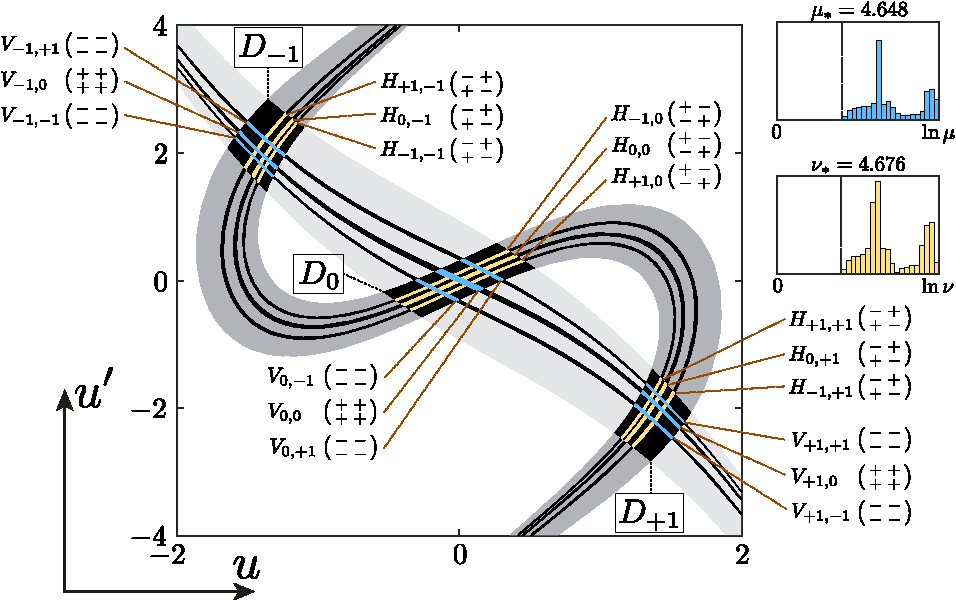
\includegraphics[width = 1\textwidth]{pic/hypotheses for piecewise equation.pdf}
	\end{figure}
\end{frame}

% ************
% * SLIDE 30 *
% ************
\begin{frame}
	\frametitle{Кусочно-постоянный псевдопотенциал: решения}
	\begin{figure}
	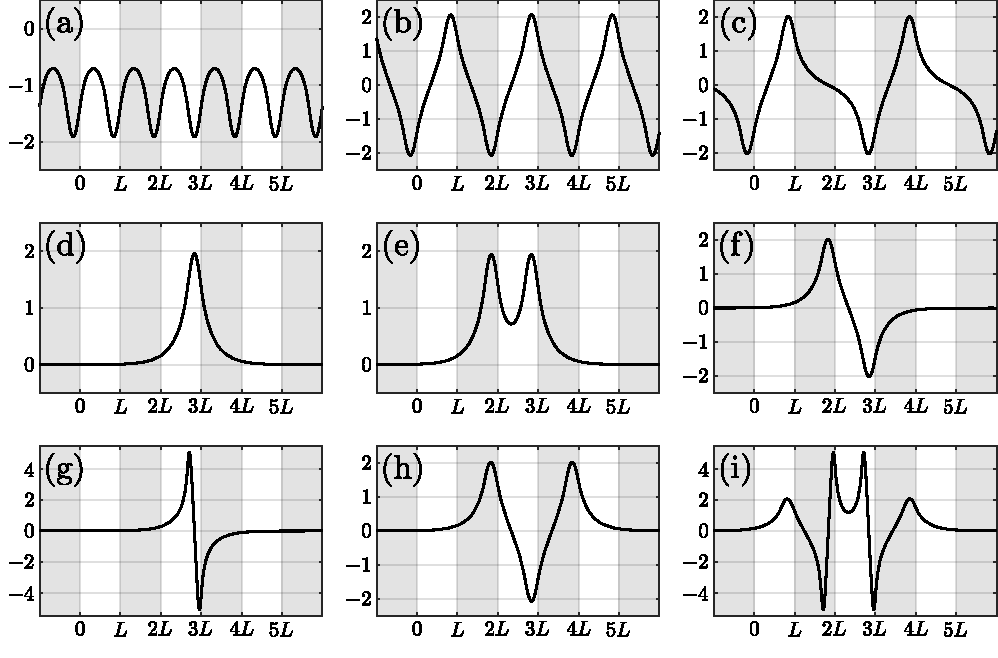
\includegraphics[width = 0.75\textwidth]{pic/solutions for piecewise equation.pdf}
	\caption{{\scriptsize
		Периодические решения: (a)~$\{ \dots, -1, -1, -1, \dots \}$; (b)~$\{ \dots, -1, +1, -1, +1 \dots \}$; (c)~$\{ \dots, -1, +1, 0, -1, +1, 0 \dots \}$.
		Локализованные решения: (d)~$\{ \dots, 0, 0, +1, 0, 0, \dots \}$; (e)~$\{ \dots, 0, 0, +1, +1, 0, 0, \dots \}$ (f)~$\{ \dots, 0, 0, +1, -1, 0, 0 \dots \}$ (g)~$\{ \dots, 0, 0, -2, 0, 0 \dots \}$ (h)~$\{ \dots, 0, 0, +1, -1, +1, 0, 0 \dots \}$ (i)~$\{ \dots, 0, 0, +1, +2, -2, +1, 0, 0 \dots \}$
	}}
	\end{figure}
\end{frame}

% ************
% * SLIDE 31 *
% ************
\begin{frame}
	\frametitle{Результаты 2-й главы}
	
	\begin{equation}
		u_{xx} + Q(x) u + P(x) u^3 = 0, \quad Q(x + L) = Q(x), \quad P(x + L) = P(x).
		\label{eq:second-chapter-results}
	\end{equation}
	
	\begin{enumerate}
		\item Предложен подход, позволяющий описать все регулярные решения уравнения \eqref{eq:second-chapter-results}.
		\item Приведены достаточные условия, дающие основания для применения подхода, а также алгоритм их численной проверки.
		\item Подход проиллюстрирован на примере уравнения \eqref{eq:second-chapter-results}, $Q(x) \equiv - 1$, $P(x) = \eta(x)$ --- кусочно-постоянный псевдопотенциал.
	\end{enumerate}
\end{frame}

% ************
% * SLIDE 32 *
% ************
\begin{frame}
	\begin{center}
		{\LARGE Глава 3. Классификация стационарных локализованных решений УГП, $$U(x) \equiv 0, \quad P(x) <> 0$$}
	\end{center}
\end{frame}

% ************
% * SLIDE 33 *
% ************
\begin{frame}
	\frametitle{Постановка задачи}
	
	\begin{equation}
		i \Psi_t + \Psi_{xx} - U(x) \Psi + P(x) |\Psi|^2 \Psi = 0.
	\label{eq:gpe-cosine}
	\end{equation}
	
	\begin{itemize}
		\item $U(x) \equiv 0$, потенциал удержания отсутствует;
		\item $P(x) = \alpha + \cos 2x$ --- периодический косинусный псевдопотенциал;
		\item $P(x) <> 0$, $\alpha \in (-1; +1)$, сингулярность --- типичное поведение решений;
		\item Стационарные решения вида $\Psi(t, x) = u(x) e^{i \omega t}$, $\omega > 0$ --- наличие локализованных решений.
	\end{itemize}
	
	\vspace{15pt}
	
	Стационарное уравнение принимает вид:
	
	\begin{equation}
		u_{xx} - \omega u + (\alpha + \cos 2x) u^3 = 0.
		\label{eq:stationary-cosine}
	\end{equation}
\end{frame}

% ************
% * SLIDE 34 *
% ************
\begin{frame}
	\frametitle{Классификация: множества $\mathscr{U}_{\pi}^{\pm}$, $\mathscr{U}_{\pi}$}
	\begin{figure}
	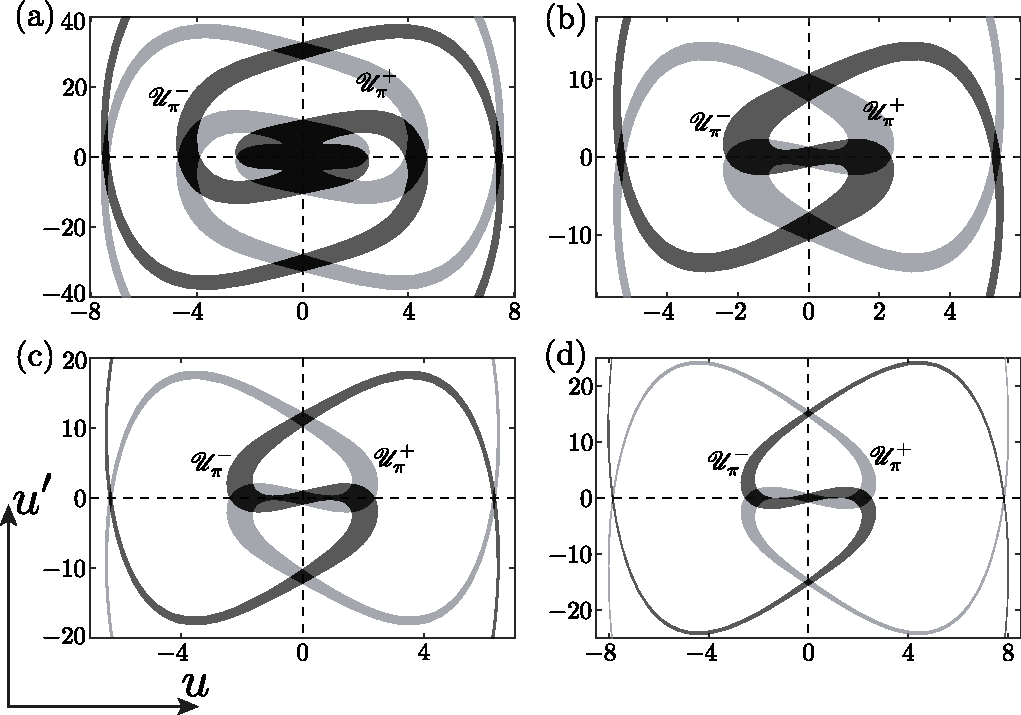
\includegraphics[width = 0.8\textwidth]{pic/island set emergence for cosine equation}
	\caption{
		Множества $\mathscr{U}_{\pi}^{\pm}$, $\mathscr{U}_{\pi} = \mathscr{U}_{\pi}^+ \cap \mathscr{U}_{\pi}^-$ для уравнения \eqref{eq:stationary-cosine}; (a)~$(\omega, \alpha) = (1, 0.6)$; (b)~$(\omega, \alpha) = (1, 0.3)$; (c)~$(\omega, \alpha) = (1, 0.1)$; (d)~$(\omega, \alpha) = (1, -0.1)$.
	}
	\end{figure}
\end{frame}

% ************
% * SLIDE 35 *
% ************
\begin{frame}
	\frametitle{Классификация: островное множество}
	
	\begin{figure}[h]
	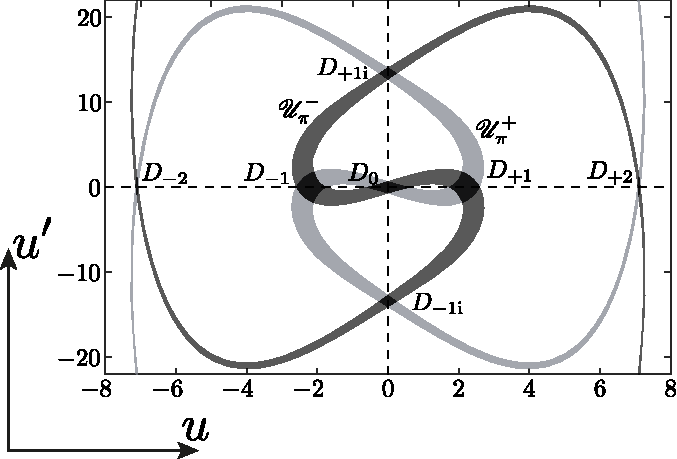
\includegraphics[width = 0.8\textwidth]{pic/island set to check hypotheses for cosine equation}
	\caption{
		Островное множество $\mathscr{U}_{\pi} = \bigcup_{k \in S_7} D_k$ (чёрный), состоящее из 7-ми островов; $(\omega, \alpha) = (1.5, 0)$.
	}
	\end{figure}
\end{frame}

% ************
% * SLIDE 36 *
% ************
\begin{frame}
	\frametitle{Классификация: проверка гипотез}
	
	\begin{figure}[h!]
	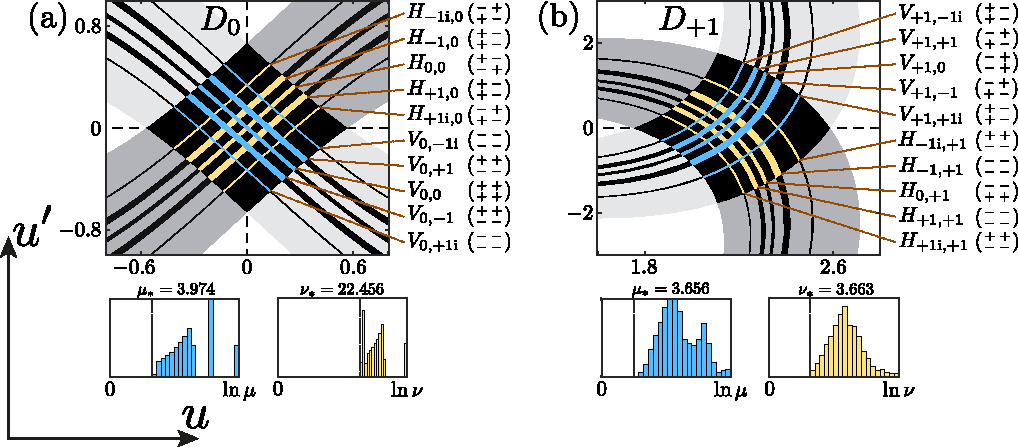
\includegraphics[width = 1\textwidth]{pic/hypotheses for cosine equation}
	\caption{Проверка гипотез для уравнения \eqref{eq:stationary-cosine} с параметрами $(\omega, \alpha) = (1.5, 0)$}
	\end{figure}
\end{frame}

% ************
% * SLIDE 37 *
% ************
\begin{frame}
	\frametitle{Классификация: решения}
	
	\begin{figure}[h]
\centering
	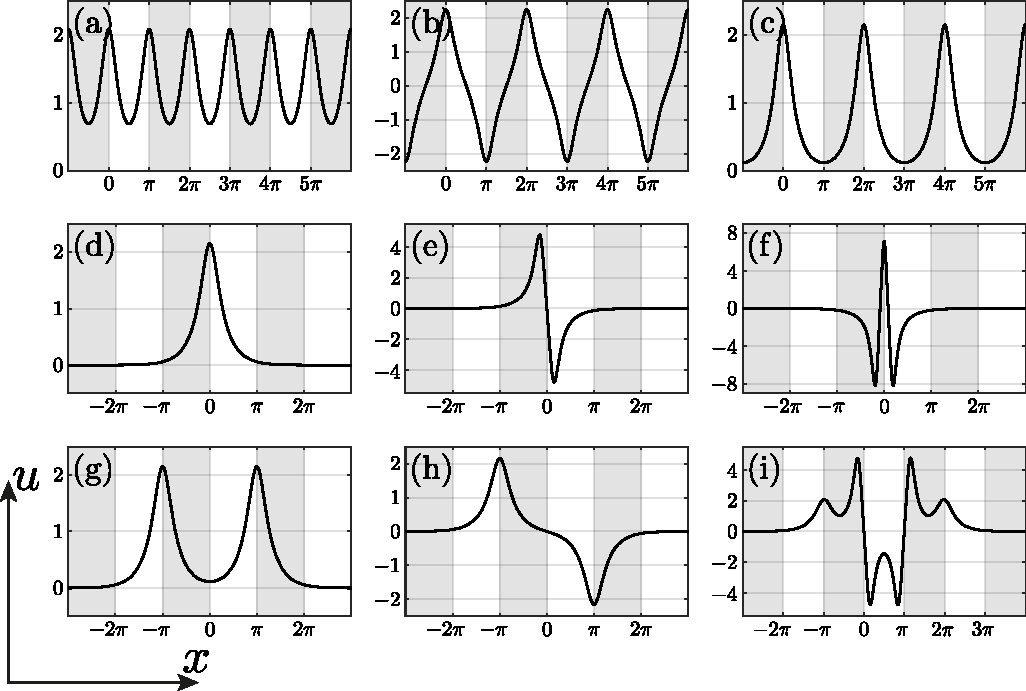
\includegraphics[width = 0.75\textwidth]{pic/solutions for cosine equation}
	\caption{{\scriptsize
		Периодические решения: (a)~$\{ \dots, +1, +1, +1, \dots \}$; (b)~$\{ \dots, +1, -1, +1, -1, \dots \}$; (c)~$\{ \dots, +1, 0, +1, 0, \dots \}$.
		Локализованные решения: (d)~фундаментальный солитон $\{ \dots, 0, +1, 0, \dots \}$; (e)~дипольный солитон $\{ \dots, 0, -1\mathrm{i}, 0, \dots \}$ (f)~$\{ \dots, 0, +2, 0, \dots \}$ (g)~$\{ \dots, 0, +1, 0, +1, 0, \dots \}$ (h)~$\{ \dots, 0, +1, 0, -1, 0, \dots \}$ (i)~$\{ \dots, 0, +1, -1\mathrm{i}, +1\mathrm{i}, +1, \dots \}$.
	}}
	\end{figure}
\end{frame}

% ************
% * SLIDE 38 *
% ************
\begin{frame}
	\frametitle{Линейная устойчивость}
	\framesubtitle{Спектральный метод}
	
	Рассматриваем малые возмущения вида
	\begin{equation}
		\Psi(t, x) = \left( u(x) + \widetilde{U}(t, x) \right) e^{i \omega t}; \quad |\widetilde{U}(t, x)| \ll 1.
	\end{equation}
	
	Линейное уравнение для возмущения $\widetilde{U}(t, x)$:
	\begin{equation}
		i \widetilde{U}_t + \widetilde{U}_{xx} - \omega \widetilde{U} + (\alpha + \cos 2x) u^2 (2 \widetilde{U} + \widetilde{U}^\dagger) = 0.
	\end{equation}

	Имещем решения в виде
	\begin{equation}
		\widetilde{U}(t, x) = (v(x) + w(x)) e^{\lambda t} + (v^{\dagger}(x) - w^{\dagger}(x)) e^{\lambda^{\dagger} t}; \quad \lambda \in \mathbb{C},
	\end{equation}
	
	Получаем задачу на собственные значения
	\begin{equation}
		i
		\begin{pmatrix}
			0 & \partial_{xx} + G_1(x) \\
			\partial_{xx} + G_2(x) & 0
		\end{pmatrix}
		\begin{pmatrix}
			v \\
			w
		\end{pmatrix}
		= \lambda 
		\begin{pmatrix}
			v \\
			w
		\end{pmatrix},
	\label{eq:eigenvalue-problem}
	\end{equation}

	\begin{eqnarray*}
		&& G_1(x) = -\omega + (\alpha + \cos 2x) u^2; \\
		&& G_2(x) = -\omega + 3 (\alpha + \cos 2x) u^2.
	\end{eqnarray*}
\end{frame}

% ************
% * SLIDE 39 *
% ************
\begin{frame}
	\frametitle{Линейная устойчивость}
	\framesubtitle{Переход к системе линейных уравнений}
	
	Рассматриваем локализованное решение на отрезке: $[-\frac{L}{2}; \frac{L}{2}]$.
	Ищем решение в пространстве Фурье:
	\begin{eqnarray}
		&& 	v(x) = \sum \limits_n a_n e^{i n k_0 x}; \quad w(x) = \sum \limits_n b_n e^{i n k_0 x}, \label{eq:eigenfunctions-expansion} \\
		&& G_1 = \sum \limits_n c_n^{(1)} e^{i n k_0 x}; \quad G_2 = \sum \limits_n c_n^{(2)} e^{i n k_0 x} \label{eq:g-functions-expansion},
	\end{eqnarray}
	где $k_0 = 2 \pi / L$.
	Подставляем \eqref{eq:eigenfunctions-expansion}, \eqref{eq:g-functions-expansion} в \eqref{eq:eigenvalue-problem}:
	 \begin{eqnarray}
		&& -(k_0 j)^2 b_j + \sum \limits_n 	c_n^{(1)} b_{j - n} = -i \lambda a_j; \\
		&& -(k_0 j)^2 a_j + \sum \limits_n 	c_n^{(2)} a_{j - n} = -i \lambda b_j,
	\end{eqnarray}
	где $-\infty < j < +\infty$.
	Рассматриваем $2N+1$ гармонику, $-N \le j \le N$.
	Получаем задачу на собственные значения \underline{линейного оператора}.
\end{frame}

% ************
% * SLIDE 40 *
% ************
\begin{frame}
	\frametitle{Линейная устойчивость: тест}
	
	\begin{center}
		Стационарное локализованное решение неустойчиво, если в спектре присутствует $\lambda$, что $\mathfrak{R}(\lambda) > 0$.
	\end{center}
	
	\begin{figure}[h!]
	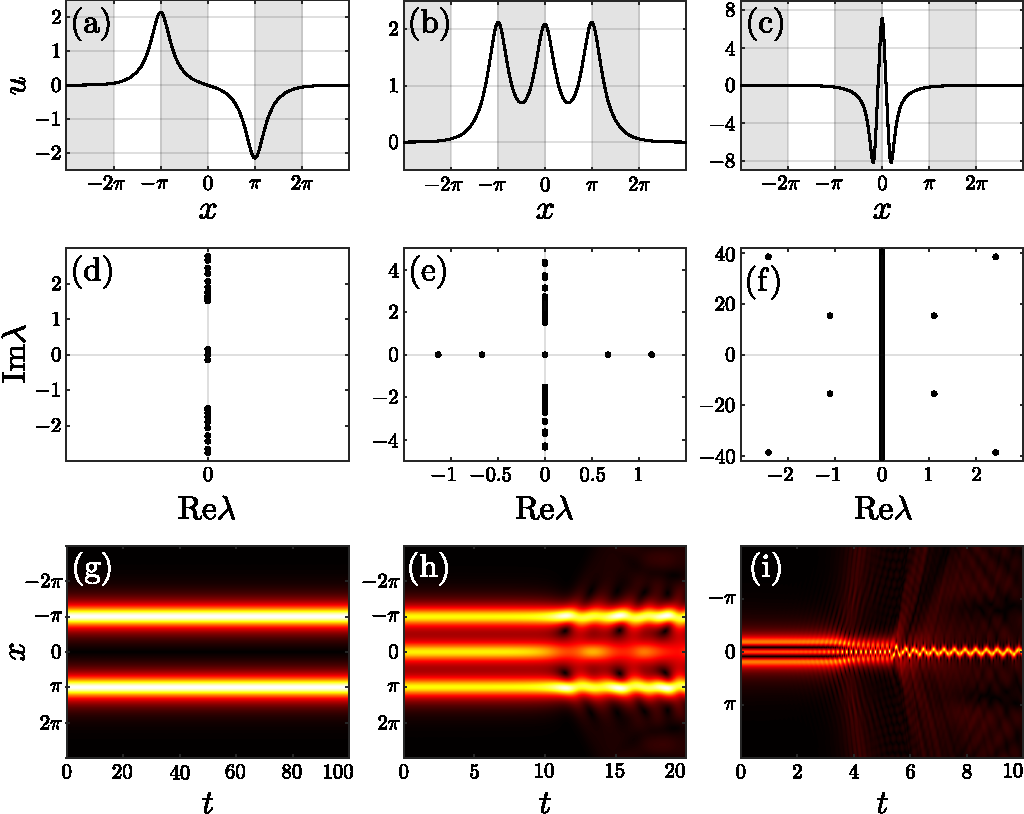
\includegraphics[width = 0.7\textwidth]{pic/stability demonstration for cosine equation}
	\end{figure}
\end{frame}

% ************
% * SLIDE 41 *
% ************
\begin{frame}
	\frametitle{Устойчивость}
	\framesubtitle{Результаты}
	
	\begin{equation}
		i \Psi_t + \Psi_{xx} + (\alpha + \cos 2x) |\Psi|^2 \Psi = 0
		\label{eq:stability-cosine}	
	\end{equation}
	
	\begin{itemize}
		\item Множество стационарных локализованных решений уравнения \eqref{eq:stability-cosine} чрезвычайно богато.
		\item Большинство их них оказываются неустойчивыми.
			Исключение составляют:
			\begin{enumerate}
				\item[1.] Фундаментальный солитон: $\{ \dots, 0, \pm 1, 0, \dots \}$.
				\item[2.] Дипольный солитон: $\{ \dots, 0, \pm 1\mathrm{i}, 0, \dots \}$ (\textcolor{forestgreen}{new}).
				\item[3.] Некоторые комбинации {\color{ceruleanblue} (1)} и {\color{ceruleanblue} (2)}: $\{ \dots, \pm 1, 0, \mp 1, 0, \dots \}$, $\{ \dots, \pm 1, \mp 1, \pm 1, 0, \dots \}$, \dots.
			\end{enumerate}
	\end{itemize}
\end{frame}

% ************
% * SLIDE 42 *
% ************
\begin{frame}
	\frametitle{Устойчивость: ветви решений}
	
	\begin{figure}[h]
	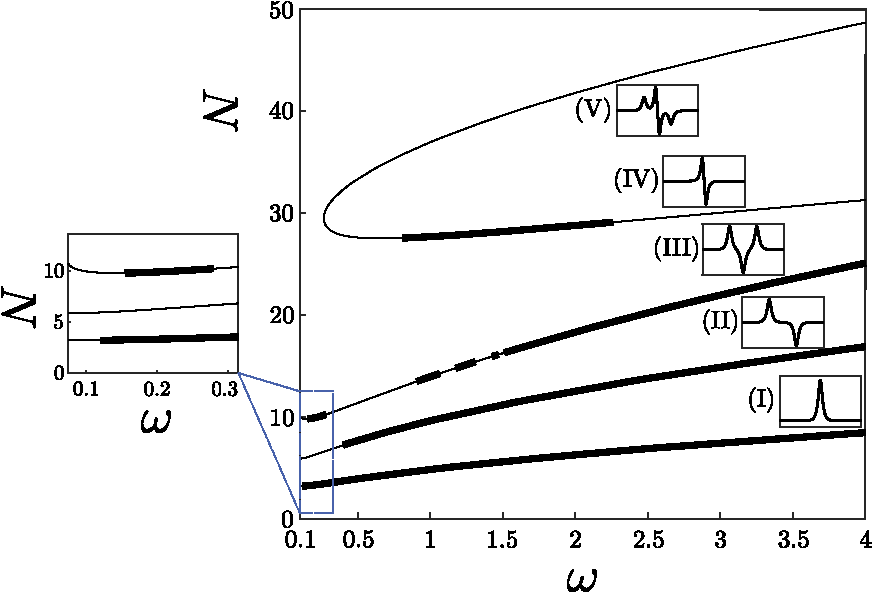
\includegraphics[width = 0.8\textwidth]{pic/branches for cosine equation}
	\caption{
		Диаграммы $N(\omega)$, для уравнения \eqref{eq:gpe-cosine}, $\alpha = 0$;
		(I)~$\{ \dots, 0, \pm 1, 0, \dots \}$; (II)~$\{ \dots, \pm 1, 0, \mp 1, 0, \dots \}$; (III)~$\{ \dots, \pm 1, \mp 1, \pm 1, 0, \dots \}$; (IV)~$\{ \dots, 0, \pm 1\mathrm{i}, 0, \dots \}$.
	}
	\end{figure}
\end{frame}

% ************
% * SLIDE 42 *
% ************
\begin{frame}
	\frametitle{Результаты 3-й главы}
	
	\begin{equation}
		i \Psi_t + \Psi_{xx} + (\alpha + \cos 2x) |\Psi|^2 \Psi = 0
		\label{eq:third-chapter-results}
	\end{equation}
	
	\begin{enumerate}
		\item Исследовано множество стационарных локализованных решений уравнения \eqref{eq:third-chapter-results}.
		\item Обнаружено новое устойчивое локализованное решение --- дипольный солитон.
	\end{enumerate}
\end{frame}

% ************
% * SLIDE 43 *
% ************
\begin{frame}
	\begin{center}
		{\LARGE Глава 4. Стационарные локализованные решения УГП в случае бесконечной потенциальной ямы и периодического псевдопотенциала, $$U(x) = Ax^2, \quad P(x) <> 0$$}
	\end{center}
\end{frame}

% ************
% * SLIDE 44 *
% ************
\begin{frame}
	\frametitle{Постановка задачи}
	
	\begin{equation}
		i \Psi_t + \Psi_{xx} - x^2 \Psi + (P_0 + P_1 \cos (\Omega x)) |\Psi|^2 \Psi = 0.
	\end{equation}
	
	Стационарные решения вида:
	\begin{equation}
		\Psi(t, x) = u(x) e^{-i \omega t}.
	\end{equation}
	
	Стационарное уравнение:
	\begin{equation}
		u_{xx} + (\omega - x^2) u + (P_0 + P_1 \cos (\Omega x)) u^3 = 0.
	\end{equation}
	
	Линейный аналог, $|u(x)| \ll 1$:
	\begin{equation}
		u_{xx} + (\omega - x^2) u = 0.
	\label{eq:ho}
	\end{equation}
	
	Решение \eqref{eq:ho} имеет вид $(\tilde{\omega}_n, \tilde{u}_n(x))$:
	\begin{equation}
		\tilde{\omega}_n = 2n + 1; \quad \tilde{u}_n(x) = \dfrac{1}{\sqrt{2^n n! \sqrt{\pi}}} H_n(x) e^{-\frac{1}{2} x^2}; \quad n = 0, 1, \dots,
	\end{equation}
	где $H_n(x)$ --- полиномы Эрмита,
	\begin{equation*}
		H_0(x) = 1, \quad H_1(x) = 2x, \quad H_2(x) = 4x^2 - 2.	
	\end{equation*}
\end{frame}

% ************
% * SLIDE 45 *
% ************
\begin{frame}
	\frametitle{Сравнение с известным случаем}
	
	Каждое решения $(\tilde{\omega}_n, \tilde{u}_n(x))$ линейной задачи бифурцирует в однопараметрическое семейство $\Gamma_n = (\omega_n, u_n(x))$ исходного уравнения.
	
	\begin{equation}
		u_{xx} + (\omega - x^2) u + \sigma_0 u^3 = 0,
	\label{eq:nho}
	\end{equation}
	
	\begin{figure}[h]
	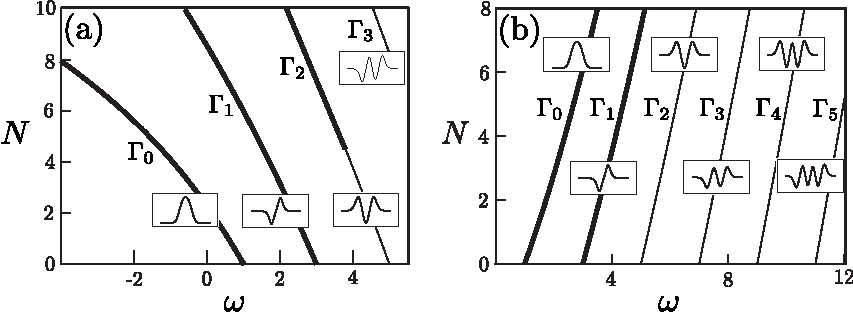
\includegraphics[width = 1\textwidth]{pic/stability for nho with constant pseudopotential}
	\caption{
		Диаграммы $N(\omega)$ семейств $\Gamma_n$ для уравнения \eqref{eq:nho}; (a) $\sigma_0 = 1$; (b) $\sigma_0 = -1$.
	}
	\label{fig:branches-nho}
	\end{figure}
	
	Все решения \eqref{eq:nho} имеют \underline{линейный аналог}.
	Других решения нет.
\end{frame}

% ************
% * SLIDE 46 *
% ************
\begin{frame}
	\frametitle{Псевдопотенциал с ненулевым средним}
	
	\begin{equation}
		u_{xx} + (\omega - x^2) u + (\sigma_0 + P_1 \cos (\Omega x)) u^3 = 0.
	\label{eq:nho-non-zero-mean}
	\end{equation}
	
	\begin{figure}[h]
	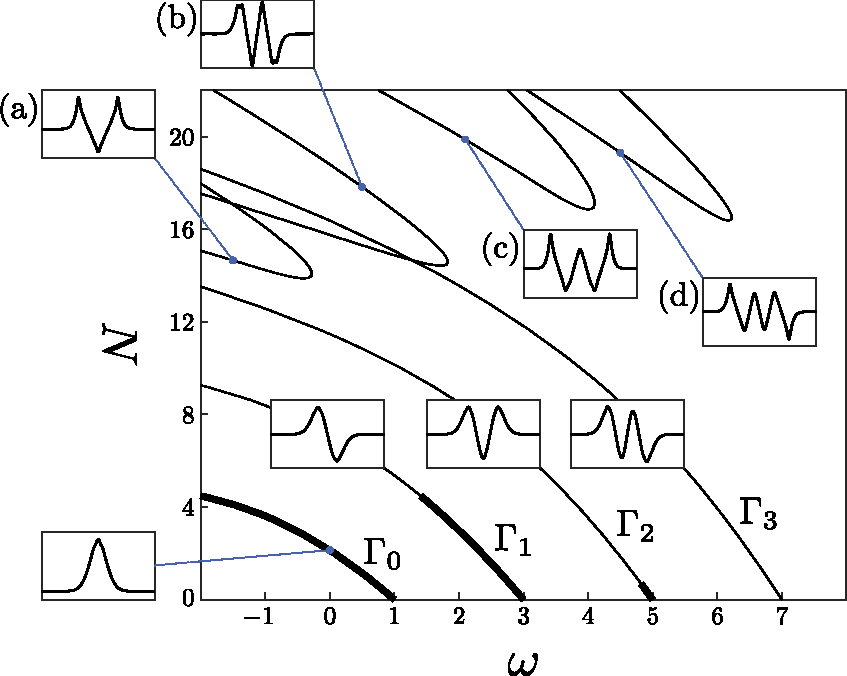
\includegraphics[width = 0.62\textwidth]{pic/branches for cosine nho, case (a)}
	\caption{
		Диаграммы $N(\omega)$ для уравнения \eqref{eq:nho-non-zero-mean} с параметрами $\sigma_0 = 1$, $P_1 = 2$, $\Omega = 12$.
	}
	\end{figure}
\end{frame}

% ************
% * SLIDE 47 *
% ************
\begin{frame}
	\frametitle{Псевдопотенциал с ненулевым средним, $\Omega \to \infty$}
	
	\begin{equation}
		u(x) = v(x) + \frac{1}{\Omega^2} \bigg( w(x) + P_1 w^3(x) \cos (\Omega x) \bigg) + o \bigg( \frac{1}{\Omega^2} \bigg), \quad \Omega \to \infty.
	\end{equation}
	
	\begin{columns}[T]
		\begin{column}{.5\textwidth}
			\begin{figure}[h]
			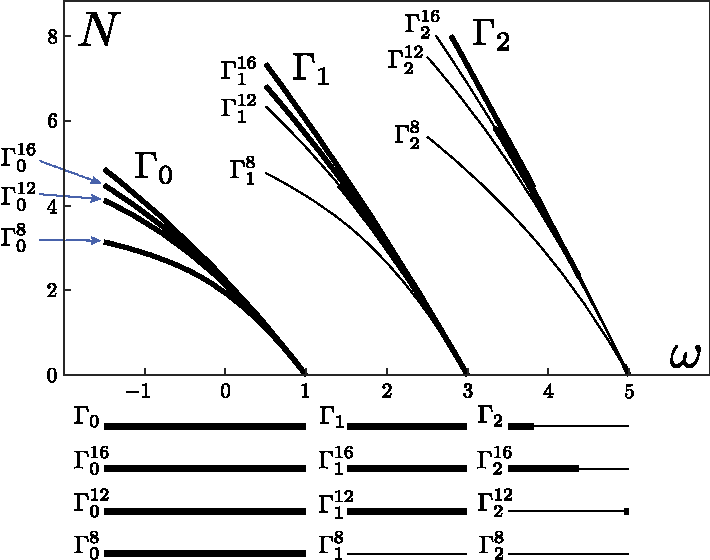
\includegraphics[width = 1\textwidth]{pic/branches with linear counterpart, non-zero mean cosine nho}
			\caption{
			Диаграммы $N(\omega)$ семейств $\Gamma_n^{\Omega}$ для уравнения \eqref{eq:nho-non-zero-mean} с параметрами $\sigma_0 = 1$, $P_1 = 2$, $\Omega = 8, 12, 16$.
			}
			\end{figure}
		\end{column}
		\begin{column}{.5\textwidth}
			\begin{figure}[h]
			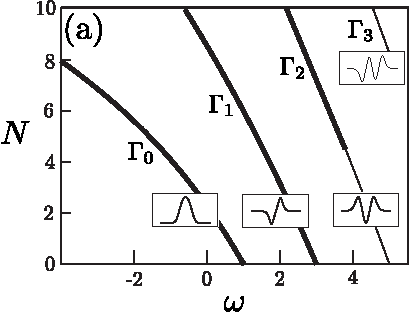
\includegraphics[width = 0.82\textwidth]{pic/stability for nho with constant pseudopotential, left}
			\caption{Диаграммы $N(\omega)$ семейств $\Gamma_n$ для уравнения с $P_1 = 0$.}
			\end{figure}
			$w(x)$ --- решение некоторого линейного уравнения.
		\end{column}
	\end{columns}
\end{frame}

% ************
% * SLIDE 48 *
% ************
\begin{frame}
	\frametitle{Псевдопотенциал с нулевым средним}
	
	\begin{equation}
		u_{xx} + (\omega - x^2) u + \sigma_1 \cos (\Omega x) u^3 = 0.
	\label{eq:nho-zero-mean}
	\end{equation}
	
	\begin{figure}[h]
	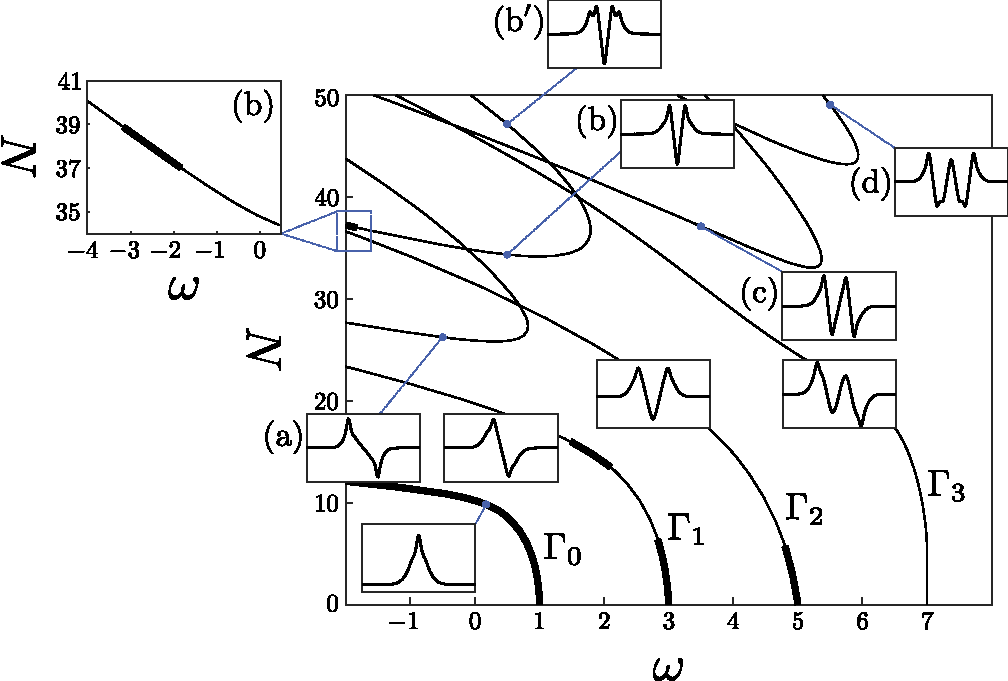
\includegraphics[width = 0.75\textwidth]{pic/branches for cosine nho, zero mean}
	\caption{
		Диаграммы $N(\omega)$ для уравнения \eqref{eq:nho-zero-mean} с параметрами $\sigma_1 = 1$, $\Omega = 8$.
	}
	\end{figure}
\end{frame}

% ************
% * SLIDE 49 *
% ************
\begin{frame}
	\frametitle{Псевдопотенциал с ненулевым средним, $\Omega \to \infty$}
	
	\begin{columns}
		\begin{column}{.5\textwidth}
			\begin{figure}[h]
			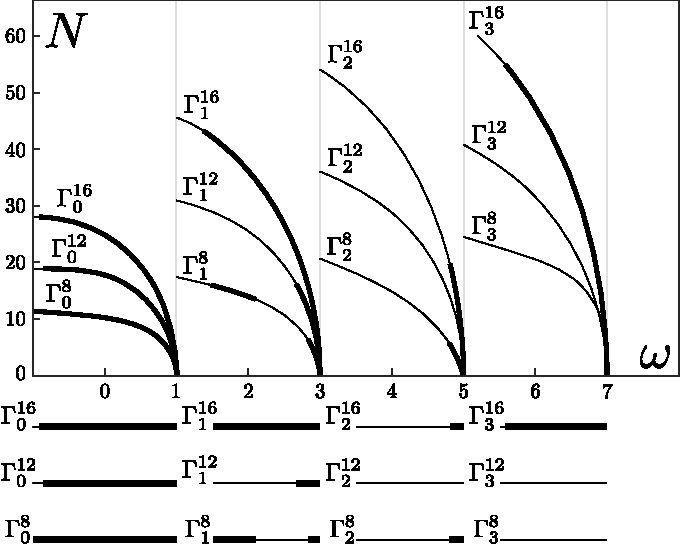
\includegraphics[width = 1\textwidth]{pic/branches with linear counterpart, zero mean cosine nho}
			\caption{
			Диаграммы $N(\omega)$ семейств $\Gamma_n^{\Omega}$ для уравнения \eqref{eq:nho-zero-mean} с параметрами $\sigma_1 = 1$, $\Omega = 8, 12, 16$.
			}
			\end{figure}
		\end{column}
		\begin{column}{.5\textwidth}
			Увеличение частоты $\Omega$ приводит к стабилизации малоамплитудных решений с линейным аналогом.
			
			\vspace{15pt}
			
			Для каждой ветви $\Gamma_n$ существует пороговое значение частоты $\Omega_n$, что для $\Omega > \Omega_n$ соответствующая ветвь решений устойчива в окрестности точки бифуркации $N \ll 1$, $\omega_n \approx \tilde{\omega}_n$.
		\end{column}
	\end{columns}
\end{frame}

% ************
% * SLIDE 50 *
% ************
\begin{frame}
	\frametitle{Результаты 4-й главы}
	
	\begin{equation}
		i \Psi_t + \Psi_{xx} - x^2 \Psi + (P_0 + P_1 \cos (\Omega x)) |\Psi|^2 \Psi = 0.
		\label{eq:fourth-chapter-results}
	\end{equation}
	
	\begin{enumerate}
		\item Присутствие периодического псевдопотенциала приводит к появлению новых классов СЛМ, не имеющих линейных аналогов.
		\item Для псевдопотенциала с нулевой средней установлено, что увеличение частоты псевдопотенциала приводит к стабилизации малоамплитудных стационарных локализованных решений.
	\end{enumerate}
\end{frame}

% ************
% * SLIDE 51 *
% ************
\begin{frame}
	\frametitle{Положения, выносимые на защиту}
	
	{\small
	\begin{enumerate}
		\item Сформулированы и доказаны общие утверждения о наличии и отсутствии сингулярных решений уравнения \eqref{eq:stationary}.
			Показано, что в случае $P(x) > 0$ все решения уравнения \eqref{eq:stationary} регулярны.
			Если $P(x)$ принимает отрицательное значение хотя бы в одной точке $x_0$, $P(x_0) < 0$, то существуют два однопараметрических семейства решений, уходящих на бесконечность в точке $x = x_0$; построена асимптотика этих решений. 
			В том случае, когда $Q(x) < 0$ и $P(x) < 0$, показано, что все решения уравнения \eqref{eq:stationary} сингулярны.
		\item Сформулированы достаточные условия возможности кодирования регулярных решений уравнения \eqref{eq:stationary} и предложен эффективный алгоритм численной проверки этих условий.
		\item Для случая $U(x) \equiv 0$, $P(x) = A + \cos 2x$ исследовано множество СЛМ уравнения \eqref{eq:gpe} и обнаружено новое устойчивое локализованное решение --- {\it дипольный солитон}.
		\item В случае бесконечной потенциальной ямы вида $U(x) = A x^2$ показано, что присутствие периодического псевдопотенциала приводит к появлению новых классов СЛМ, не имеющих аналогов в моделях с $P(x) = \mathrm{const}$.
			Для псевдопотенциала с нулевым средним установлено, что частота псевдопотенциала существенным образом влияет на устойчивость СЛМ.
			Установлено, что увеличение частоты приводит к стабилизации малоамплитудных стационарных локализованных решений.
	\end{enumerate}
	}
\end{frame}

% ************
% * SLIDE 52 *
% ************
\begin{frame}
	\frametitle{Публикации}
	
	\begin{large}
	{
		\color{ceruleanblue}
		10 публикаций, \\
		3 статьи, индексируемые системой Scopus.
	}	
	\end{large}

	\medskip

	% Rework with some bibliography style approach.
	\begin{scriptsize}
	\begin{enumerate}
		\setlength\itemsep{10pt}
		\item[1.] Алфимов Г. Л., Лебедев М. Е., <<О регулярных и сингулярных решениях уравнения>> $u_{xx} + Q(x) u + P(x) u^3 = 0$ // Уфимск. матем. журн. том {\bf 7}, выпуск 2, стр. 3--18 (2015).
		\item[2.] Lebedev M. E., Alfimov G. L., Malomed B. A., ``Stable dipole solitons and soliton complexes in the nonlinear Schr\"odinger equation with periodically modulated nonlinearity'' // Chaos: An Interdisciplinary Journal of Nonlinear Science {\bf 26} (7), 073110 (2016).
		\item[3.] G. L. Alfimov, L. A. Gegel, M. E. Lebedev, B. A. Malomed, and D. A. Zezyulin, ``Localized modes in the Gross-Pitaevskii equation with a parabolic trapping potential and a nonlinear lattice pseudopotential'' // Communications in Nonlinear Science and Numerical Simulation {\bf 66}, 194–207 (2019).
		\item[4.] G. L. Alfimov, M. E. Lebedev, ``Coding of stationary modes for the nonlinear Schrödinger equation with periodically modulated nonlinearity'' // International Conference ``Hamiltonian Dynamics, Nonautonomous Systems, and Patterns in PDE's'', Lobachevsky State University of Nizhni Novgorod, Nizhni Novgorod, December 2014.
		\item[5.] Алфимов Г. Л., Лебедев М. Е., <<Стационарные моды нелинейного уравнения Шрёдингера в присутствии линейного и нелинейного потенциалов>> // Мат. конф. <<Фундаментальная математика и ее приложения в естествознании>>, БашГУ, Уфа, сентябрь 2015.
	\end{enumerate}
	\end{scriptsize}
\end{frame}

% ************
% * SLIDE 53 *
% ************
\begin{frame}
	\frametitle{Публикации}
	\begin{scriptsize}
	\begin{enumerate}
		\setlength\itemsep{10pt}
		\item[6.] M. E. Lebedev, G. L. Alfimov, B. A. Malomed, ``Stable dipole solitons and soliton complexes in the nonlinear Schrödinger equation with periodically modulated nonlinearity'' // International Conference ``Dynamics, Bifurcations and Chaos III'', Lobachevsky State University of Nizhni Novgorod, Nizhni Novgorod, July 2016.
		\item[7.] G. L. Alfimov, L. A. Gegel, M. E. Lebedev, D. A. Zezyulin, B. A. Malomed, ``Steady-states for the Gross-Pitaevskii equation with nonlinear lattice pseudopotential'' // International Conference ``Complex Analysis, Mathematical Physics and Nonlinear Equations'', Bashkortostan, Bannoe Lake, March 2018.
		\item[8.] G. L. Alfimov, M. E. Lebedev, D. A. Zezyulin, B. A. Malomed, ``Steady-states for the Gross-Pitaevskii equation with nonlinear lattice pseudopotential'' // International Conference ``Nonlinear Phenomena in Bose Condensates and Optical Systems'', Tashkent, Uzbekistan, August 2018.
		\item[9.] Lebedev M. E., Shipitsyn K. V., ``Coding of solutions for the Duffing equation with non-homogeneous nonlinearity'' // International Conference ``Complex Analysis, Mathematical Physics and Nonlinear Equations'', Bashkortostan, Bannoe Lake, March 2019.
		\item[10.] M. E. Lebedev, G. L. Alfimov, ``Coding of bounded solutions of equation $u_{xx} - u + \eta(x) u^3 = 0$ with periodic piecewise constant function $\eta(x)$'' // International Conference ``Complex Analysis, Mathematical Physics and Nonlinear Equations'', Bashkortostan, Bannoe Lake, March 2021.
	\end{enumerate}
	\end{scriptsize}
\end{frame}

% ************
% * SLIDE 54 *
% ************
\begin{frame}
	\begin{center}
		{\Huge Спасибо за внимание!}
	\end{center}
\end{frame}
	
\end{document}
